\documentclass[10pt,a4paper]{article}
\usepackage[utf8]{inputenc}
\usepackage{amsmath}
\usepackage{amsfonts}
\usepackage{amssymb}
\usepackage{graphicx}
\usepackage{epstopdf}
\usepackage{inputenc}
\usepackage{geometry}
\usepackage{graphicx}
\usepackage[normalem]{ulem}
\usepackage{hyperref}
\usepackage[dvipsnames]{xcolor}
\usepackage{subcaption}
\hypersetup{
    colorlinks=false, %set true if you want colored links
    linktoc=all,     %set to all if you want both sections and subsections linked 
}
\author{Author: \textcolor{MidnightBlue}{\href{https://www.linkedin.com/in/simone-staffa-8b3b79158}{Simone Staffa}}}
\title{{\Huge\textbf{Process and Service Design}
\\ \LARGE Professor: Pierluigi Plebani
\begin{figure}[h!]
 \hfill 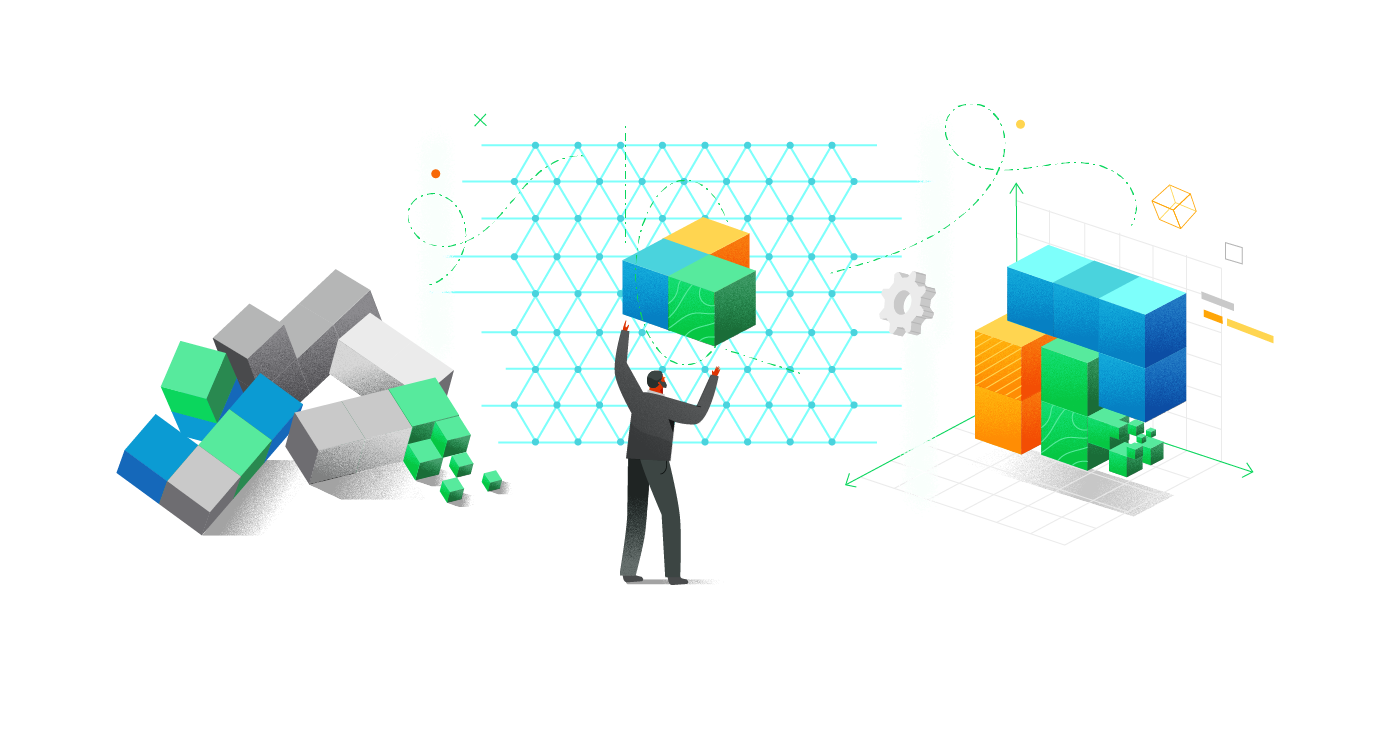
\includegraphics[width=200pt]{images/cover.png}\hspace*{\fill}
  \label{fig:polimi}
\end{figure} \\
}}
\date{Politecnico di Milano \\ Computer Science $\&$ Engineering | Fall 2019-2020}
\newcommand{\myparagraph}[1]{\paragraph{#1}\mbox{}\\[0.05in]}
\newcommand{\mydefinition}[1]{\textcolor{MidnightBlue}{\textit{"#1"}\\ \\}}
\begin{document}
\maketitle
\clearpage
\tableofcontents
\clearpage
\section{\LARGE Introduction}
The meaning of term \textbf{service} is intuitive but is definition can be different in different contexts like:
\begin{itemize}
	\item Economic
	\item ICT
\end{itemize}
We firstly need to understand similarities and differences among these different terms:
\begin{itemize}
	\item Service
	\item e-Service
	\item Web-Service
\end{itemize}
\uline{Definition of service}: \\
\textit{“A service is a change in the condition of a person, or a good belonging to some economic unit, which is brought about as the result of the activity of some other economic unit, with the prior agreement of the former person or economic unit".  (P. Hill, On goods and services)} \\
\begin{figure}[h!]
  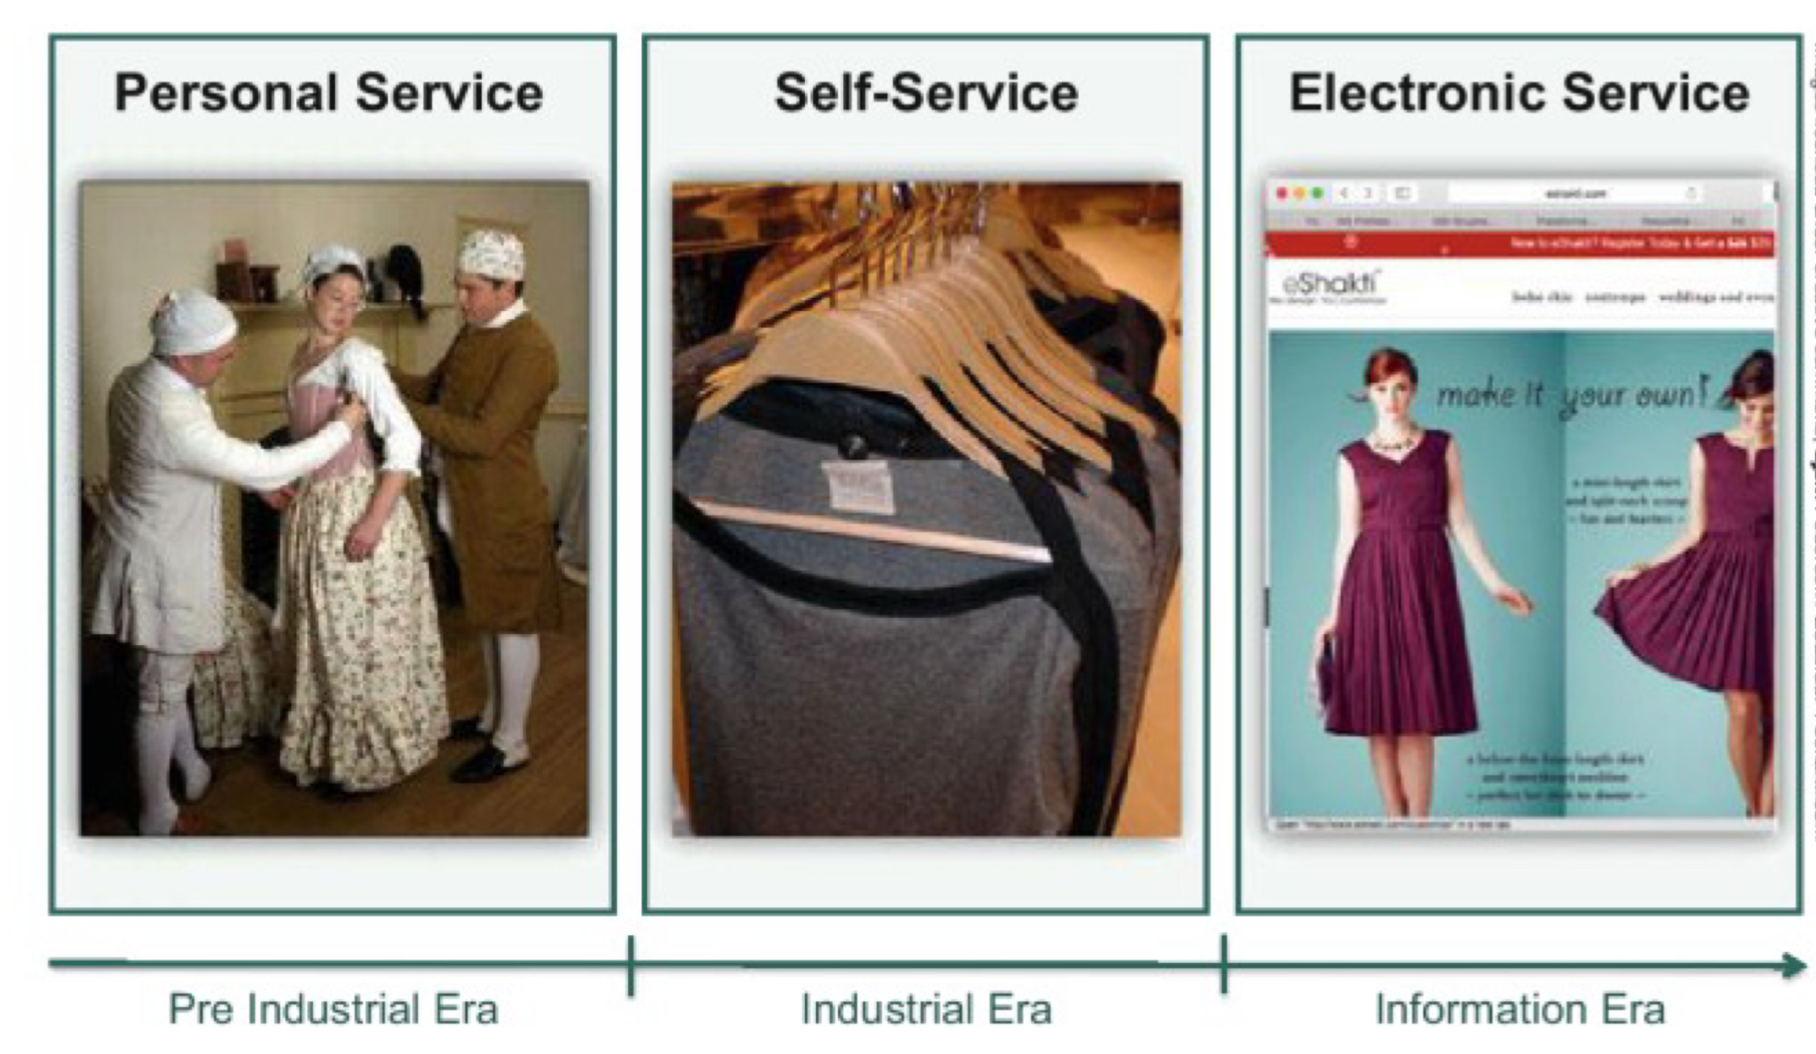
\includegraphics[width=\linewidth]{images/services-types}
  \caption{Looking for a dress, in different eras}
  \label{fig:buffer-manager}
\end{figure} \\
The above picture represents the evolution of the services along the years. Specially, it refers to the dress service. In the Pre Industrial era was more like a personal service, where a tailors offered totally customized dresses to people directly in their houses. Then with the Industrial Era, dresses were sold by retailer, so the final product was not really customized by the consumers, who just had to select the already made dress they liked. Finally, nowadays in the Information Era, service started to be offered through IT Platforms, with full customization without even the need to go to the shop, dresses can be just bought and received at home.\\
This can be also applied to the IT domain, for what we call nowadays Web Services. \\
The Pre Industrial Era corresponds to when people used to build their own computers, buying different parts and installing them by their selves. The Industrial Era corresponds to when companies started building personal computers to be sold to consumers, who just had to pay and bring them home. Finally, the Information Era corresponds to nowadays Cloud Platform and Web Services that allow people to rent virtual computers online, to perform their own computation. \\ \\
Just to recap:
\begin{itemize}
	\item \textbf{Personal service (Pre Industrial era)}: highly and man-made customization but limited production
	\item \textbf{Industrial service (Industrial era)}: mass production but no customization
	\item \textbf{Electronic service (Information era)}: highly and computer-based customization combined with mass production
\end{itemize}
This to say that we are \textbf{evolving to a service-oriented society}. \\
\uline{\textit{"We don't need a drill, we need a hole in the wall."}} \\ \\ 
From an economic perspective, we are switching from a Good-dominant logic to a Service-dominant logic.
\begin{itemize}
	\item \textbf{Good-dominant logic} focuses on goods exchange, that's why goods are considered to be tangible and each of them has an embedded value that is taken into account to operate exchange transactions.
	\item \textbf{Service-dominant logic} focuses on service provision, where resources are  intangible and require a co-creation of value.
\end{itemize}
S-D logic is useful because it opens to more interactions with customers and allows to focus on why a product fits to the customer needs instead of technical specification. \\ \\
When technology comes into play, there are two different perspectives of ICT in S-D logic, which go under the name of e-Service.
\begin{itemize}
	\item As the improvement of a programming paradigm
	\begin{itemize}
		\item \textbf{ICT is a goal} and it is offered itself as a service
		\item SOA (Service Oriented Architecture) becomes the new way of developing software to be service-ready
		\end{itemize}
\item As the automation of economics activities and self-service
	\begin{itemize}
		\item \textbf{ICT is a mean} and can improve the effectiveness and the efficacy
		\item The goal is to make the business able to provide services
	\end{itemize}
\end{itemize}
As a mean, ICT has a fundamental role in the evolution towards the S-D logic. Who deliver products must pay a lot of attention on Customization, Scalability, Reliability and Security/Privacy. \\
As a goal, ICT is also a service to be delivered and a possible way to deliver these service could be using a Web Service.
\section{\LARGE Service Definition}
\end{document}